\chapter{Wobbling Motion Study via a Boson Description}
\label{extra-chapter-new-boson}

The last part will be focused on the same wobbling phenomenon but with a different approach than the ones employed in Chapters \ref{chapter-4-aw1-formalism} and \ref{chapter-5-novel}, as this method does not share the same foundational concepts as the $\mathbf{W_1}$ and $\mathbf{W_2}$ techniques. The results shown here correspond to a recent publication made by the team in Ref. \cite{raduta2020new}. The structure of the chapter is organized as follows: in the first section a set of results achieved by the $\mathbf{W_0}$ formalism are briefly recalled, as some key features from that work will be used throughout this chapter. 
%TO-DO: finish summary of chapter 6.

\section{Angular Momentum - Boson Representation}
\label{section-intro-boson-representation}

Besides the odd-mass case-study performed by the team in Ref. \cite{raduta2017semiclassical}, the first part consisted in describing wobbling motion for even-even nuclei using a \emph{boson expansion} of the angular momentum components. The problem considered a triaxial rigid rotor with moments of inertia $\mathcal{I}_k$, which described by the known rotor Hamiltonian (recall Section \ref{trm-model} and Eq. \ref{general-rotor-hamiltonian}):
\begin{align}
    \hat{H}_R=\frac{\hat{R}_1}{2\mathcal{I}_1}+\frac{\hat{R}_2}{2\mathcal{I}_2}+\frac{\hat{R}_3}{2\mathcal{I}_3}\ ,
\end{align}
and angular momentum components $\hat{R}_k$. From this initial quantal problem, a variational principle (similar recipe as the one described in Section \ref{variational-principle-section}, but only for one set of coordinates) brings the system into a classical view, where the eigenvalue problem becomes a system of classical equations in a phase space (see Section II.A and II.B from Ref. \cite{raduta2017semiclassical}). Summarizing the calculations, one obtained $i)$ a pair of conjugate variables (i.e., $r$ and $\varphi$) and $ii)$ two equations of motion (recall discussion from Section \ref{equations-of-motion-section} and Eq. \ref{eq-of-motion-approach-w1}) as:
\begin{align}
    \frac{\partial\mathcal{H}}{\partial r}=\dot{\varphi}\ ,\ \frac{\partial\mathcal{H}}{\partial\varphi}=-\dot{r}\ ,
\end{align}
with $\mathcal{H}$ as the average of $\hat{H}_R$ with the trial function. If the average values of the angular momentum components are expressed in terms of the phase space coordinates $(r,\varphi)$, then the following equations emerge:
\begin{align}
    J_+^\text{cls}&\equiv\langle\hat{R}_+\rangle=\sqrt{r(2I-r)}e^{\iu\varphi}\ ,\nonumber \\
    J_-^\text{cls}&\equiv\langle\hat{R}_-\rangle=\sqrt{r(2I-r)}e^{-\iu\varphi}\ ,\nonumber \\
    J_3^\text{cls}&\equiv\langle\hat{R}_3\rangle=r-I\ .
    \label{classical-am-components-boson}
\end{align} 

Their algebra being governed by the Poisson brackets, which defines their inner product:
\begin{align}
    \left\{J_+^\text{cls},J_-^\text{cls}\right\}=-2\iu J_3^\text{cls}\ ,\ \left\{J_\pm^\text{cls},J_3^\text{cls}\right\}=\pm\iu J_{\pm}^\text{cls}\ .
    \label{classical-J-poisson-brackets}
\end{align} 

The three functions $J_+^\text{cls}$, $J_-^\text{cls}$, $J_3^\text{cls}$ together with the Poisson brackets from Eq. \ref{classical-J-poisson-brackets} generate a classical algebra $\left[\text{SU}(2)\right]_\text{cls}$. A pair of complex functions $f$ and $g$ defined in this classical phase space will have their associated Poisson bracket:
\begin{align}
    \left\{f,g\right\}=\frac{\partial f}{\partial \varphi}\frac{\partial g}{\partial r} - \frac{\partial f}{\partial r}\frac{\partial g}{\partial \varphi}\ .
\end{align} 

The classical coordinates belonging to that phase space were then re-quantized through the \emph{Dyson boson expansion} \cite{dyson1956general}, which signified a change of the picture from the classical $\left[\text{SU}(2)\right]_\text{cls}$ back to a quantized view. Firstly, the quantization starts with two canonical complex variables written in terms of the conjugate coordinates $(r, \varphi)$:
\begin{align}
    \mathcal{C}=\sqrt{2I}\sqrt{r^{-1}(2I-r)}e^{-\iu\varphi}\ ,\nonumber\\
    \mathcal{B}^*=\sqrt{2I}^{-1}\sqrt{r(2I-r)}e^{\iu\varphi}\ ,
    \label{complex-variables-dyson}
\end{align}
and the Poisson bracket:
\begin{align}
    \left\{\mathcal{B}^*,\mathcal{C}\right\}=\iu\ .
\end{align}

The quantization process within the Dyson representation implies that a new set of quantal operators $b$ and $b^\dagger$ should replace the two complex coordinates, and the inner product defined by the Poisson bracket becomes the commutator operator:
\begin{align}
    \left(\mathcal{C},\mathcal{B}^*,\{,\}\right)\Longrightarrow\left(b,b^\dagger,-\iu \left[,\right]\right)\ .
    \label{dyson-transformation}
\end{align} 

The transformation employed in Eq. \ref{dyson-transformation} will introduce the following set of angular momentum components:
\begin{align}
    \hat{J}_+^\text{D}&=\sqrt{2I}b^\dagger\ ,\nonumber\\
    \hat{J}_-^\text{D}&=\sqrt{2I}\left(1-\frac{b^\dagger b}{2I}\right)b\ ,\nonumber\\
    \hat{J}_3^\text{D}&=I-b^\dagger b\ .
    \label{dyson-boson-expansion-am-components}
\end{align}

The set of angular momentum components $\hat{J}^\text{D}$ provided in Eq. \ref{dyson-boson-expansion-am-components} marks the onset of the Dyson boson representation. A function that depends on the variables from Eq. \ref{complex-variables-dyson} can be quantized by first writing its expression in terms of $\mathcal{C}$ and $\mathcal{B}^*$ and then replace both variables by the boson operators $b$ and $b^\dagger$. The transformation is boson like because of the nature of $b$ and $b^\dagger$. These operators obey the boson canonical commutation relations:
\begin{align}
    \left[b,b^\dagger\right]=1\ ,\ \left[b,b\right]=\left[b^\dagger,b^\dagger\right]=0\ .
    \label{boson-commutation-relations}
\end{align}

The classical energy function $\mathcal{H}$ can be written in terms of the variables $\mathcal{C}$ and $\mathcal{B}$ and then replace them with the boson operators $b$ and $b^\dagger$. Consequently, the Dyson representation of the rotor Hamiltonian $\hat{H}_R$ is obtained, which was denoted by $\hat{H}_D$. The search for \emph{real} eigenvalues for $\hat{H}_D$ was made through the \emph{Bargmann representation} \cite{bargmann1962representations,jancovici1964collective,janssen1971boson}. This mapping associates to the operators $b,b^\dagger$ two differential operators, which leads to a differential equation for $\hat{H}_D$:
\begin{align}
    b^\dagger\rightarrow x\ ,\ b\rightarrow \frac{d}{dx}\ .
    \label{bargmann-mapping-equation}
\end{align}

Indeed, by using the mapping from Eq. \ref{bargmann-mapping-equation}, the eigenvalue problem becomes equivalent with solving the second order differential equation (recall Eq. 2.34 from Ref. \cite{raduta2017semiclassical}):
\begin{align}
    \left[p(x^4)\frac{d^2}{dx^2}+q(x^3)\frac{d}{dx}-r(x^2)\right]G=E'G\ .
\end{align}

Further calculations from that work gave the energy spectrum for $^{158}$Er, providing unique results for the even-even deformed nuclei. The \emph{transitions} from a quantal space ($\hat{H}_R$) to a classical space ($\mathcal{H}$), and then a re-quantized ($\hat{H}_D$) showed some remarkable features of the approach. In all three cases, a great agreement with the experimental data was obtained for the yrast band the first two excited bands. The fact that the semi-classical treatment gives similar results with quantal (and, inherently, more complex) methods was a key result that emerged from $\mathbf{W_0}$.

\section{Theoretical Framework}
\label{section-new-boson-theoretical-framework}

The boson representation of the angular momentum operator was introduced in Section \ref{section-intro-boson-representation} since the work from Ref. \cite{raduta2020new} is based on such representations. In this paper, the team proposed a novel formalism, which is based on the idea of expanding the angular momentum components in terms if boson operators. In contrast to $\mathbf{W_0}$, here the even-odd mass nuclei are considered. By using the Bargmann mapping, the eigenvalue equation associated to the model Hamiltonian is brought to a Schrödinger-like structure. In addition, a harmonic approximation performed on this equation will lead to some analytical formulas for the wobbling frequency.

\subsection{Potential Energy for thr PRM Hamiltonian}

Since the initial problem consists of an odd-$A$ nucleus, the particle-triaxial rotor Hamiltonian is adopted. A rigid-coupling approximation is considered, meaning that the angular momentum of the odd particle is aligned with the core. The Hamiltonian for the system will become (keeping the notations consistent with the work from Ref. \cite{raduta2020new}):
\begin{align}
    \hat{H}_\text{rot}=\sum_{k}A_k\left(\hat{I}_k-\hat{j}_k\right)^2\ ,
    \label{rotor-hamiltonian-new-boson}
\end{align}
where $k=1,2,3$, and $A_k$ is the inertia factor (used throughout the previous chapters). As per the \emph{rigid coupling}, the single-particle a.m. $\mathbf{j}$ will stay in the principal plane $(1,2)$, meaning that the vector is described by $\mathbf{j}=\left(j\cos\theta,j\sin\theta,0\right)$. In addition, the largest MOI is considered the one along the 2-axis (i.e., $\mathcal{I}_2$). In a first-order approximation, the angular momentum component $\hat{I}_2$ can be expanded as:
\begin{align}
    \hat{I}_2=I\left(1-\frac{1}{2}\frac{\hat{I}_1^2+\hat{I}_3^2}{I^2}\right)\ ,
\end{align}
and through this expansion, the Hamiltonian from Eq. \ref{rotor-hamiltonian-new-boson} can be rewritten as:
\begin{align}
    \hat{H}_\text{rot}=A\hat{H}'+\left(A_1I^2-A_2j_2\right)+\sum_{k=1,2}A_k\hat{j}_k^2\ .
    \label{rewritten-rotor-hamiltonian-new-boson}
\end{align}

In this equation, the following notations have been adopted:
\begin{align}
    \hat{H}'&=\hat{I}_2^2+u\hat{I}_3^2+2v_0\hat{I}_1\ ,\nonumber\\
    u&=\frac{A_3-A_1}{A}\ ,\nonumber\\
    v_0&=-\frac{A_1j_1}{A}\ ,\nonumber\\
    A&=A_2\left(1-\frac{j_2}{I}\right)-A_1\ ,\nonumber\\
    A&>0\ ,\ -1<u<1\ .
    \label{new-boson-hamiltonian-notations}
\end{align}

Taking a closer look at the Hamiltonian depicted in Eq. \ref{rewritten-rotor-hamiltonian-new-boson}, it can be seen that $\hat{H}'$ looks like the triaxial rotor Hamiltonian, but amended with a new term, which would act as a constraint on the system (\emph{cranking-like term}), making it rotate around the one-axis. In this research, the cranking axis is set to be $1$-axis. Following the same recipe as in the $\mathbf{W_0}$ case, the a.m. components are expressed in terms of the raising and lowering operators:
\begin{align}
    \hat{I}_\pm=\hat{I}_2\pm\iu\hat{I}_3\ ,\ \hat{I}_0=\hat{I}_1\ .
\end{align}

The a.m. components satisfy the commutation relations (in the rotating reference frame):
\begin{align}
    \left[\hat{I}_-,\hat{I}_+\right]=2\hat{I}_0\ ,\ \left[\hat{I}_\mp,\hat{I}_0\right]=\mp\hat{I}_\mp\ .
\end{align}

Using these variables, the expression of $\hat{H}'$ from Eq. \ref{new-boson-hamiltonian-notations} becomes:
\begin{align}
    \hat{H}'=\frac{1-u}{4}\left(\hat{I}_+^2+\hat{I}_-^2\right)+\frac{1+u}{4}\left(\hat{I}_+\hat{I}_-+\hat{I}_-\hat{I}_+\right)+2v_0\hat{I}_0\ .
    \label{hamiltonian-new-boson-ladder-operators}
\end{align}

For this Hamiltonian, the Schrödinger equation:
\begin{align}
    \hat{H}'\ket{\Psi}=E\ket{\Psi}\ ,
\end{align}
is expressed in terms of two conjugate variables $q$ and $d/dq$ with the help of a special representation of the angular momentum components. Indeed, by using the Jacobi Elliptic functions $\text{sn}$ ($s$), $\text{cn}$ ($c$), and $\text{dn}$ ($d$), respectively \cite{jacobi1829fundamenta,akhiezer1990elements}. These functions are used quite often in physics, especially in non-linear problems \cite{kovacic2016jacobi} and are defined as:
\begin{align}
    s&\equiv\text{sn}(q,k)\ ,\ c\equiv\text{cn}(q,k)\ ,\ d\equiv\text{dn}(q,k)\ ,\nonumber\\
    k&=\sqrt{|u|}\ ,\ k'=\sqrt{1-k^2}\ ,\nonumber\\
    q&=\int_0^\varphi \frac{1}{\sqrt{1-k^2\sin^2(x)}}dx\equiv F(\varphi,k)\ .
    \label{elliptic-functions-equation}
\end{align}

An alternative representations for the elliptic functions is in terms of the trigonometric functions:
\begin{align}
    s=\sin\varphi\ ,\ c=\cos\varphi\ ,\ d=\sqrt{1-k^2s^2}\ .
\end{align}
The behavior of $s$, $c$, and $d$ is graphically shown in Fig. \ref{elliptic-functions-plot}. It can be observed that these functions are periodic, with the periods $4K$, $4K$, and $2K$, respectively. The value of $K$ is given by replacing $\varphi=\pi/2$ in $F(\varphi,k)$ from Eq. \ref{elliptic-functions-equation}.
\begin{figure}
    \centering
    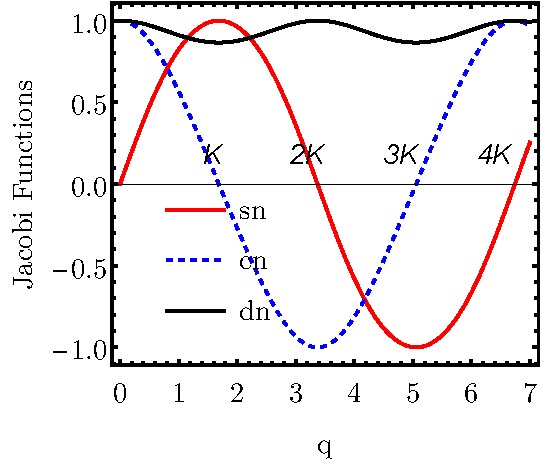
\includegraphics[scale=1]{Chapters/Figures/Jacobi-Elliptic-Functions.pdf}
    \caption{The elliptic functions sn, cd, and dn from Eq. \ref{elliptic-functions-equation} are represented as functions of $q$. The value of the \emph{elliptic modulus} $k$ is set to $1/2$.}
    \label{elliptic-functions-plot}
\end{figure}